\documentclass[10pt]{article}
\usepackage[letterpaper,margin=0.9in,bottom=0.7in]{geometry}
\usepackage{amsmath,amssymb}
\usepackage{graphicx}
\usepackage{setspace}
\usepackage[T1]{fontenc}
\pagestyle{empty}
\setlength{\parindent}{0pt}
\setlength{\parskip}{0.32em}
\setstretch{1.02}

\begin{document}
\enlargethispage{4\baselineskip}

\begin{center}
{\large\bfseries How Many Local Epochs? Communication Cost and\\
Variable Selection in Federated Lasso}\\[0.55em]
Keivan Bolouri\\[0.15em]
{\footnotesize Department of Statistics, Donald Bren School of Information and Computer Sciences\\
University of California, Irvine
\quad\textbullet\quad
\texttt{kbolouri@uci.edu}}
\end{center}

\vspace{0.15em}

\noindent\textbf{Problem.}
Multi-site pharmaceutical research increasingly depends on data that cannot be centralized ---
records behind institutional firewalls, trials under separate data-use agreements, claims databases no single
sponsor controls. Federated learning shares model parameters, not patient records. When the goal is
\textit{which variables matter} --- candidate biomarkers, covariates for a safety model --- the natural tool is a sparse
regression such as the Lasso. Every federated protocol must choose $E$, the number of local update steps
each site takes between aggregation rounds; larger $E$ buys fewer communication rounds but risks client
drift. For coordinate descent on the Lasso the concern is specific: because the $\ell_1$ penalty zeros coordinates
by soft-thresholding, drift can lead sites to prune different predictors --- the damage appears as a different
variable list, not merely a worse fit.

\noindent\textbf{Setup.}
We evaluate a synchronous federated coordinate-descent Lasso on a high-dimensional continuous-response
regression dataset whose data-generating process and true coefficient vector were not disclosed to the
analyst, so a centralized Lasso on the pooled sample serves as the reference rather than a known support
(data and code: \texttt{github.com/KeivanBolouri/federated-lasso}).
The training sample ($n = 800$, $p = 600$) is partitioned into $K = 3$ disjoint sites with
$m_j = 400, 240, 160$, so variation across sites arises from the partition rather than from distinct data
sources. Each site selects its penalty on its own validation split from a 30-point log-scale grid; the pooled
reference is fitted with the same grid and criterion on the pooled validation split, so both sides of the
comparison are tuned by the same rule. Each site then runs $E$ full coordinate-descent passes per round
and the server aggregates by sample-size weight; no row-level data are exchanged during federated fitting.
We sweep $E\in\{1, 2, 3, 5, 8, 10, 15, 20\}$, recording rounds, upload cost, and agreement between the
federated active set and that reference (197 active predictors).

\noindent\textbf{Results.}
Recall against the reference falls monotonically from 86.3\% to 69.5\% as $E$ grows from 1 to 20,
while precision stays flat (42.8--46.2\%). However, F1 and Jaccard are not monotone: both peak at $E=3$
(0.583, 0.412), above their values at $E=1$ (0.572, 0.401). Moving from $E=1$ to $E=3$ cuts rounds from 27
to 13 and upload from 379.7 to 182.8~KiB --- a 52\% reduction --- while slightly improving agreement with
the centralized fit, so the two objectives did not conflict in this range in this run. Beyond $E=5$, upload
cost continues to decline while F1 and Jaccard generally decrease; $E=15$ and $E=20$ both require six
rounds and 84.4~KiB of upload, although their support-agreement metrics differ slightly. At $E=10$ the
federated model matches 137 of the 197 reference predictors against 170 at $E=1$ --- the same data yielding
a materially different candidate list.

\vspace{0.05em}
\begin{center}
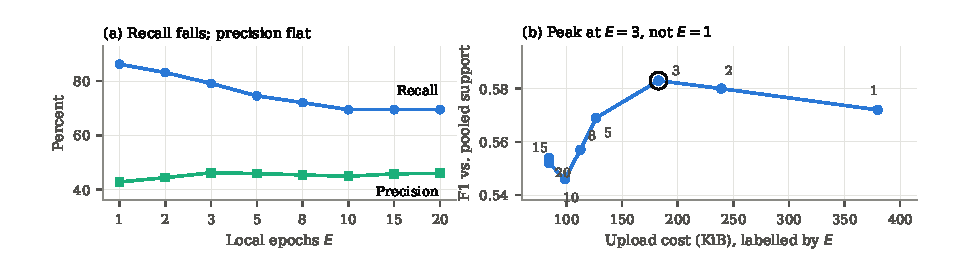
\includegraphics[width=0.92\textwidth]{figure1.pdf}\\[0.05em]
{\scriptsize\textbf{Figure 1:} Recall declines monotonically in $E$ while precision is flat (a), so agreement with the centralized fit peaks in the interior at $E=3$ rather than at $E=1$ (b). In this single run, reducing communication from $E=1$ to $E=3$ did not reduce observed F1.}
\end{center}

\noindent\textbf{Implication.}
A preliminary coarse grid $\{1, 5, 10\}$ favored $E=5$ on final penalized objective (25.8165
against 25.8906 at $E=1$), missing the $E=2$--$3$ region entirely. Objective and selection metrics disagreed
about which schedule was best, suggesting the penalized objective alone may be insufficient for choosing $E$
when support stability matters.

\noindent\textbf{Limitations.}
Results come from a single draw of one dataset with no error bars, so the $E=1$ versus
$E=3$ gap is not separated from sampling noise, and the data are not multi-site clinical data --- the framing
above is motivation, not demonstrated performance. With the true support unknown, the metrics measure
agreement with an estimated reference, not correctness. The recall pattern is consistent with client drift,
though drift was not measured directly, and no baseline comparison (FedProx, SCAFFOLD, ADMM) is
included; replication and those comparisons are in progress.

\end{document}
